\subsection{Spændingsforsyning} \label{test_spaendingsforsyning}
Det forventes, at spændingsforsyningen leverer en konstant spænding til EMG-forstærkeren, så denne fungerer optimalt, og så EMG-signalerne ikke forstyrres. For at undersøge, om spændingsforsyningen opfylder de opstillede krav i \ref{sec:krav_spaending}, testes spændingsforsyningen med et multimeter, hvor outputspændingen måles. %Ét kabel tilsluttes $V_{cc}$, og ét andet tilsuttes ground. 
Ud fra dette er den positive spænding målt til $5,574~V$ og den negative spænding til $-5,341~V$, hvilket giver en peak-to-peak-amplitude på $10,815~V$. Under testen, blev der ikke set udslag på multimeteret, hvorved spændingsforsyningen overholder kravet om at skulle kunne levere en jævn spænding. Dette betyder at spændingsforsyningen kan udsende en spænding, som er passede for at forsyne EMG-forstærkeren, der typisk kræver en spænding på typisk $\pm3V$, jf. \autoref{sec:EMG_krav}. 
Derudover testets der for om spændingsregulatoren udsender et signal, hvis den ikke leverer en konstant spændingen. Dokumentation for denne test fremgår  af \autoref{fig:spaendingsforsyning_LED}. Det blev målt at spændingsregulatoren leverede en spænding på omkring $\pm5,4~V$ når LED'en var tændt, mens den leverede en spænding på $0,0985~mV$ når LED'en var slukket.


\begin{figure}[H]
\centering
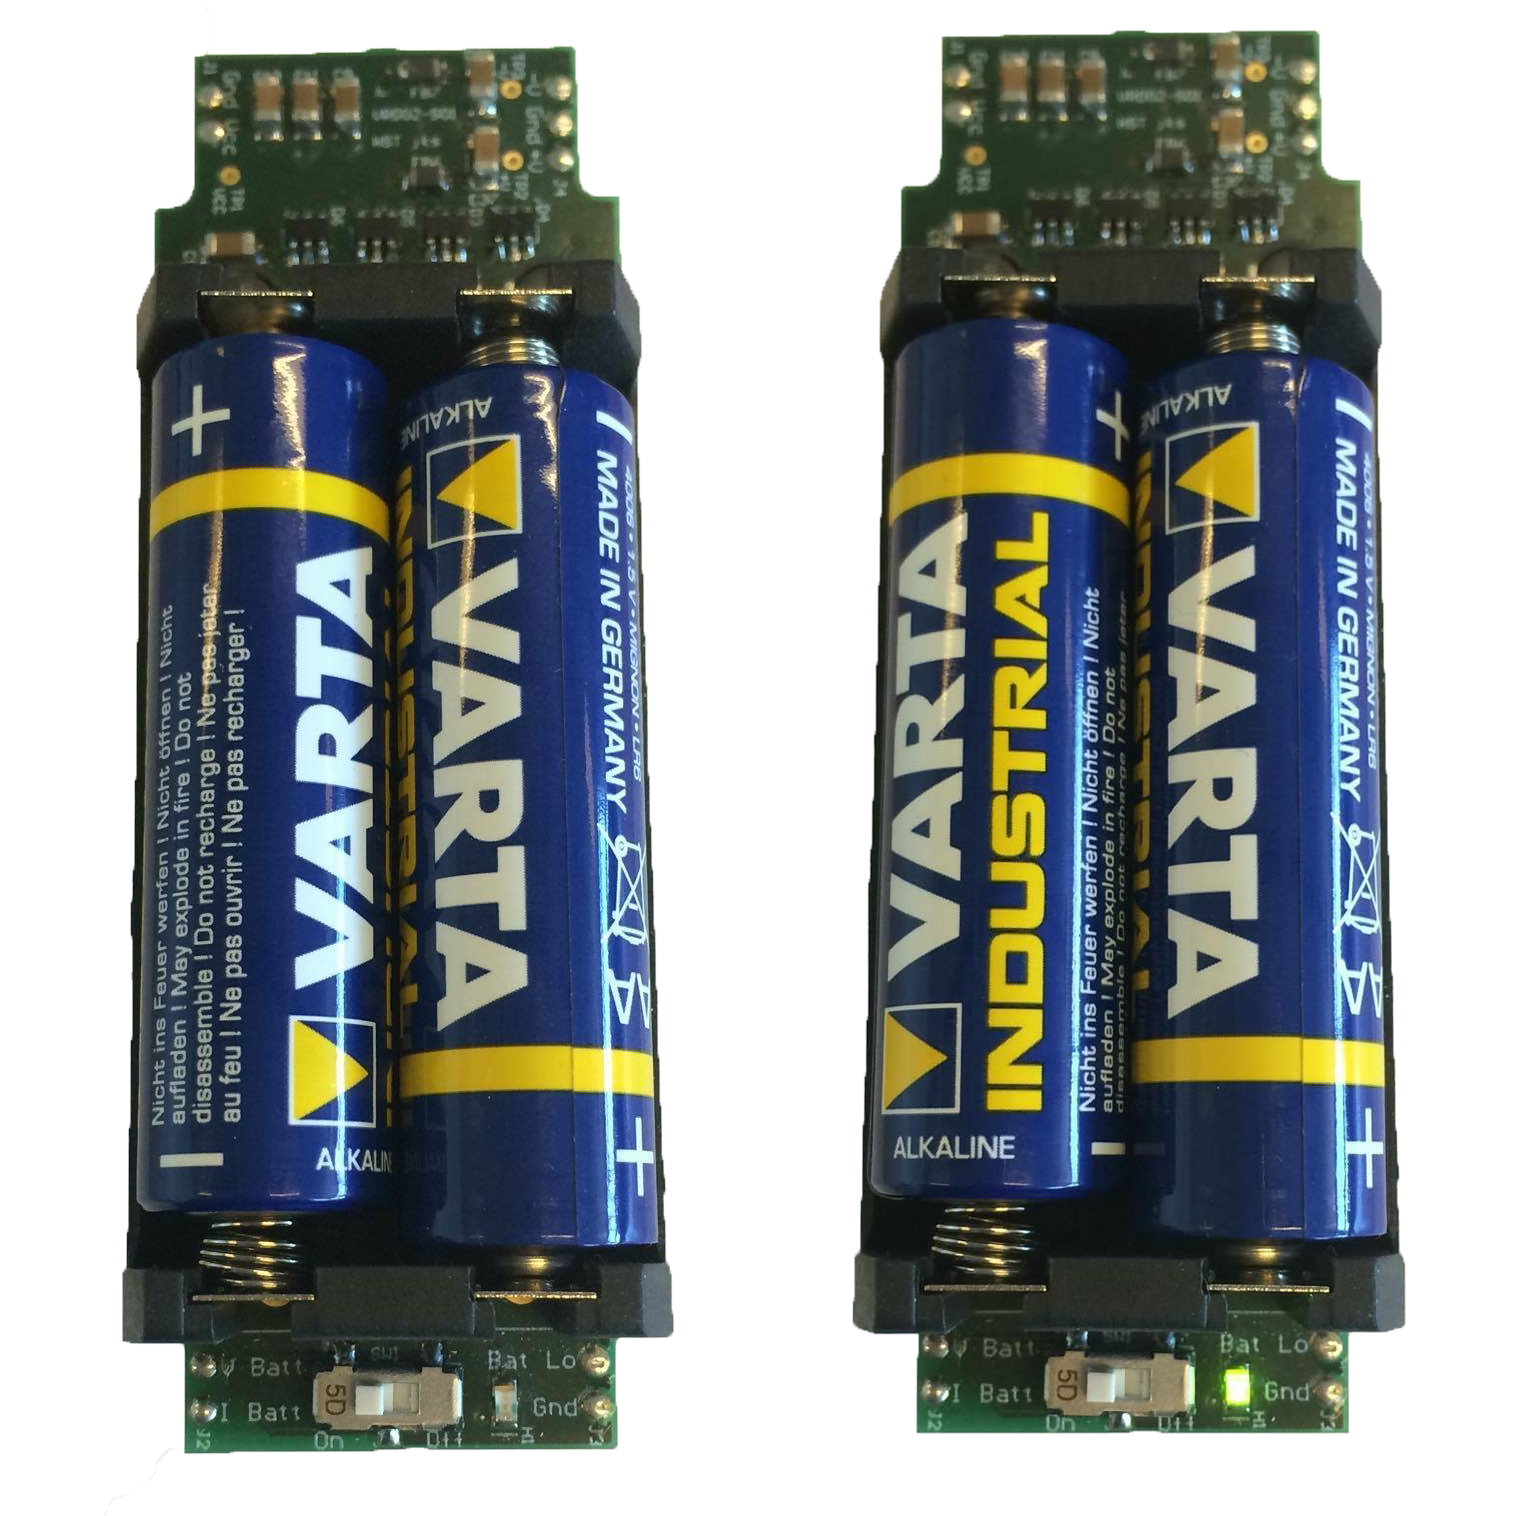
\includegraphics[width=0.6\textwidth]{figures/bat_test}
\caption{Billedet til højre viser spændingsregulatorens når den leverer en spænding på $5,4~V$, hvorved en LED lyser grønt for indikere dette. Billedet til venstre viser spændingsregulatoren når den ikke leverer en passende spænding, hvormed LED'en er slukket.}
\label{fig:spaendingsforsyning_LED}
\end{figure}


